\documentclass[twoside]{book}

% Packages required by doxygen
\usepackage{fixltx2e}
\usepackage{calc}
\usepackage{doxygen}
\usepackage[export]{adjustbox} % also loads graphicx
\usepackage{graphicx}
\usepackage[utf8]{inputenc}
\usepackage{makeidx}
\usepackage{multicol}
\usepackage{multirow}
\PassOptionsToPackage{warn}{textcomp}
\usepackage{textcomp}
\usepackage[nointegrals]{wasysym}
\usepackage[table]{xcolor}

% Font selection
\usepackage[T1]{fontenc}
\usepackage[scaled=.90]{helvet}
\usepackage{courier}
\usepackage{amssymb}
\usepackage{sectsty}
\renewcommand{\familydefault}{\sfdefault}
\allsectionsfont{%
  \fontseries{bc}\selectfont%
  \color{darkgray}%
}
\renewcommand{\DoxyLabelFont}{%
  \fontseries{bc}\selectfont%
  \color{darkgray}%
}
\newcommand{\+}{\discretionary{\mbox{\scriptsize$\hookleftarrow$}}{}{}}

% Page & text layout
\usepackage{geometry}
\geometry{%
  a4paper,%
  top=2.5cm,%
  bottom=2.5cm,%
  left=2.5cm,%
  right=2.5cm%
}
\tolerance=750
\hfuzz=15pt
\hbadness=750
\setlength{\emergencystretch}{15pt}
\setlength{\parindent}{0cm}
\setlength{\parskip}{3ex plus 2ex minus 2ex}
\makeatletter
\renewcommand{\paragraph}{%
  \@startsection{paragraph}{4}{0ex}{-1.0ex}{1.0ex}{%
    \normalfont\normalsize\bfseries\SS@parafont%
  }%
}
\renewcommand{\subparagraph}{%
  \@startsection{subparagraph}{5}{0ex}{-1.0ex}{1.0ex}{%
    \normalfont\normalsize\bfseries\SS@subparafont%
  }%
}
\makeatother

% Headers & footers
\usepackage{fancyhdr}
\pagestyle{fancyplain}
\fancyhead[LE]{\fancyplain{}{\bfseries\thepage}}
\fancyhead[CE]{\fancyplain{}{}}
\fancyhead[RE]{\fancyplain{}{\bfseries\leftmark}}
\fancyhead[LO]{\fancyplain{}{\bfseries\rightmark}}
\fancyhead[CO]{\fancyplain{}{}}
\fancyhead[RO]{\fancyplain{}{\bfseries\thepage}}
\fancyfoot[LE]{\fancyplain{}{}}
\fancyfoot[CE]{\fancyplain{}{}}
\fancyfoot[RE]{\fancyplain{}{\bfseries\scriptsize Generated by Doxygen }}
\fancyfoot[LO]{\fancyplain{}{\bfseries\scriptsize Generated by Doxygen }}
\fancyfoot[CO]{\fancyplain{}{}}
\fancyfoot[RO]{\fancyplain{}{}}
\renewcommand{\footrulewidth}{0.4pt}
\renewcommand{\chaptermark}[1]{%
  \markboth{#1}{}%
}
\renewcommand{\sectionmark}[1]{%
  \markright{\thesection\ #1}%
}

% Indices & bibliography
\usepackage{natbib}
\usepackage[titles]{tocloft}
\setcounter{tocdepth}{3}
\setcounter{secnumdepth}{5}
\makeindex

% Hyperlinks (required, but should be loaded last)
\usepackage{ifpdf}
\ifpdf
  \usepackage[pdftex,pagebackref=true]{hyperref}
\else
  \usepackage[ps2pdf,pagebackref=true]{hyperref}
\fi
\hypersetup{%
  colorlinks=true,%
  linkcolor=blue,%
  citecolor=blue,%
  unicode%
}

% Custom commands
\newcommand{\clearemptydoublepage}{%
  \newpage{\pagestyle{empty}\cleardoublepage}%
}

\usepackage{caption}
\captionsetup{labelsep=space,justification=centering,font={bf},singlelinecheck=off,skip=4pt,position=top}

%===== C O N T E N T S =====

\begin{document}

% Titlepage & ToC
\hypersetup{pageanchor=false,
             bookmarksnumbered=true,
             pdfencoding=unicode
            }
\pagenumbering{alph}
\begin{titlepage}
\vspace*{7cm}
\begin{center}%
{\Large Meanshift \\[1ex]\large 1.\+0 }\\
\vspace*{1cm}
{\large Generated by Doxygen 1.8.13}\\
\end{center}
\end{titlepage}
\clearemptydoublepage
\pagenumbering{roman}
\tableofcontents
\clearemptydoublepage
\pagenumbering{arabic}
\hypersetup{pageanchor=true}

%--- Begin generated contents ---
\chapter{Mean shift implementation}
\label{index}\hypertarget{index}{}\begin{DoxyAuthor}{Author}
Damir Demirović \href{mailto:damir.demirovic@untz.ba}{\tt damir.\+demirovic@untz.\+ba}
\end{DoxyAuthor}
Mean shift algorithm represent a general non-\/parametric mode finding procedure. It\textquotesingle{}s a hill-\/climbing algorithm on the density defined by a finite mixture or a kernel density estimate. Mean shift can be used as a non-\/parametric clustering method, for object tracking, image segmentation. 
\chapter{Todo List}
\label{todo}
\Hypertarget{todo}

\begin{DoxyRefList}
\item[\label{todo__todo000001}%
\Hypertarget{todo__todo000001}%
File \hyperlink{io__png_8c}{io\+\_\+png.c} ]handle lossless 16bit data 

add a test suite 

internally handle R\+G\+B/gray conversion in io\+\_\+png\+\_\+read\+\_\+raw() 

handle deinterlacing as a libpng transform function 
\item[\label{todo__todo000003}%
\Hypertarget{todo__todo000003}%
Member \hyperlink{io__png_8c_a54ce4037b9759d9a8f31c01d3315821d}{io\+\_\+png\+\_\+read\+\_\+u8} (const char $\ast$fname, size\+\_\+t $\ast$nxp, size\+\_\+t $\ast$nyp, size\+\_\+t $\ast$ncp)]don\textquotesingle{}t downscale 16bit images. 
\item[\label{todo__todo000005}%
\Hypertarget{todo__todo000005}%
Member \hyperlink{io__png_8c_a8b49182e70dfd843d7bafbc7a5278172}{io\+\_\+png\+\_\+write\+\_\+f32} (const char $\ast$fname, const float $\ast$data, size\+\_\+t nx, size\+\_\+t ny, size\+\_\+t nc)]handle 16bit images and flexible min/max
\end{DoxyRefList}
\chapter{Class Index}
\section{Class List}
Here are the classes, structs, unions and interfaces with brief descriptions\+:\begin{DoxyCompactList}
\item\contentsline{section}{\hyperlink{structMSPoint}{M\+S\+Point} }{\pageref{structMSPoint}}{}
\end{DoxyCompactList}

\chapter{File Index}
\section{File List}
Here is a list of all documented files with brief descriptions\+:\begin{DoxyCompactList}
\item\contentsline{section}{src/\hyperlink{meanshift_8cpp}{meanshift.\+cpp} \\*Main program for Meanshift segmentation }{\pageref{meanshift_8cpp}}{}
\item\contentsline{section}{src/\hyperlink{msfilter_8cpp}{msfilter.\+cpp} \\*Main program for Meanshift filtering }{\pageref{msfilter_8cpp}}{}
\item\contentsline{section}{src/image/\hyperlink{image_8cpp}{image.\+cpp} \\*Image helper functions }{\pageref{image_8cpp}}{}
\item\contentsline{section}{src/image/{\bfseries image.\+h} }{\pageref{image_8h}}{}
\item\contentsline{section}{src/io\+\_\+png/\hyperlink{io__png_8c}{io\+\_\+png.\+c} \\*P\+NG read/write simplified interface }{\pageref{io__png_8c}}{}
\item\contentsline{section}{src/io\+\_\+png/{\bfseries io\+\_\+png.\+h} }{\pageref{io__png_8h}}{}
\item\contentsline{section}{src/ms/\hyperlink{ms_8cpp}{ms.\+cpp} \\*Functions for Meanshift algorithm }{\pageref{ms_8cpp}}{}
\item\contentsline{section}{src/ms/{\bfseries ms.\+h} }{\pageref{ms_8h}}{}
\item\contentsline{section}{src/ra/{\bfseries R\+A\+List.\+h} }{\pageref{RAList_8h}}{}
\item\contentsline{section}{src/ra/{\bfseries Transitive\+Closure.\+h} }{\pageref{TransitiveClosure_8h}}{}
\end{DoxyCompactList}

\chapter{Class Documentation}
\hypertarget{structMSPoint}{}\section{M\+S\+Point Struct Reference}
\label{structMSPoint}\index{M\+S\+Point@{M\+S\+Point}}
\subsection*{Public Attributes}
\begin{DoxyCompactItemize}
\item 
\mbox{\Hypertarget{structMSPoint_ac2152817f66a26328ac254faa75e3152}\label{structMSPoint_ac2152817f66a26328ac254faa75e3152}} 
int {\bfseries x}
\item 
\mbox{\Hypertarget{structMSPoint_a69f9951f757c44d02a1eadae7c5fb025}\label{structMSPoint_a69f9951f757c44d02a1eadae7c5fb025}} 
int {\bfseries y}
\end{DoxyCompactItemize}


The documentation for this struct was generated from the following file\+:\begin{DoxyCompactItemize}
\item 
src/ms/ms.\+h\end{DoxyCompactItemize}

\chapter{File Documentation}
\hypertarget{image_8cpp}{}\section{src/image/image.cpp File Reference}
\label{image_8cpp}\index{src/image/image.\+cpp@{src/image/image.\+cpp}}


Image helper functions.  


{\ttfamily \#include \char`\"{}image.\+h\char`\"{}}\newline
{\ttfamily \#include $<$cstdlib$>$}\newline
Include dependency graph for image.\+cpp\+:\nopagebreak
\begin{figure}[H]
\begin{center}
\leavevmode
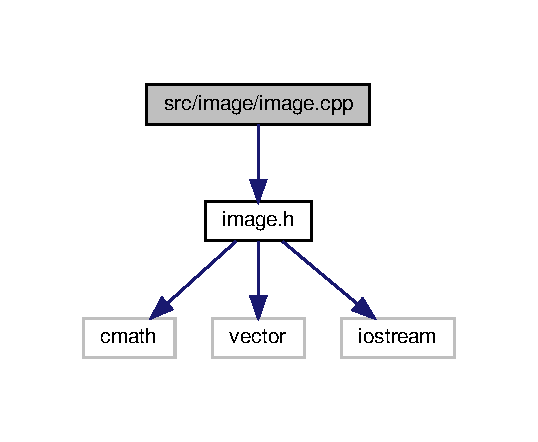
\includegraphics[width=258pt]{image_8cpp__incl}
\end{center}
\end{figure}
\subsection*{Functions}
\begin{DoxyCompactItemize}
\item 
uchar $\ast$ \hyperlink{image_8cpp_aaf269bff7c09327eea93a955e3680b8d}{Allocate\+Uchar\+Image} (int width, int height, int nchannel)
\begin{DoxyCompactList}\small\item\em Allocate space for the uchar image,. \end{DoxyCompactList}\item 
int $\ast$$\ast$ \hyperlink{image_8cpp_a1ed8d4f7fb14a60d16b27ae7fd8b1661}{Generate\+Labels} (size\+\_\+t width, size\+\_\+t height)
\begin{DoxyCompactList}\small\item\em Generate labels for clustering. \end{DoxyCompactList}\item 
vector$<$ int $>$ \hyperlink{image_8cpp_a9db41200e4b9be68cc2809d733920e8f}{Generate\+Random\+Numbers} (int count)
\begin{DoxyCompactList}\small\item\em Function generate random numbers. \end{DoxyCompactList}\item 
void \hyperlink{image_8cpp_aeb43573df64a948fbf767dfc5a9e6e10}{Label\+Image} (uchar $\ast$image, int width, int height, int $\ast$$\ast$labels, int reg\+Count)
\begin{DoxyCompactList}\small\item\em Function Label\+Image in R\+GB colors. \end{DoxyCompactList}\item 
void \hyperlink{image_8cpp_abd4d6fd513a32dd7c6cb87a9fd55ee93}{R\+G\+B2\+L\+UV} (float r, float g, float b, uchar $\ast$l, uchar $\ast$u, uchar $\ast$v)
\begin{DoxyCompactList}\small\item\em Function R\+G\+B2\+L\+UV converts R\+GB pixel value to L\+UV pixel value. \end{DoxyCompactList}\item 
void \hyperlink{image_8cpp_a098aa7f739868f62e83e20c4ea7dfb94}{L\+U\+V2\+R\+GB} (float L, float u, float v, uchar $\ast$R, uchar $\ast$G, uchar $\ast$B)
\begin{DoxyCompactList}\small\item\em Function L\+U\+V2\+R\+GB converts L\+UV pixel value to R\+GB pixel value. \end{DoxyCompactList}\item 
uchar $\ast$ \hyperlink{image_8cpp_a74f85606f0ad784c0874d52cfafe6271}{Convert\+R\+G\+B2\+L\+UV} (uchar $\ast$rgb, int width, int height, int nchannel)
\begin{DoxyCompactList}\small\item\em Function Convert\+R\+G\+B2\+L\+UV convert R\+GB image to L\+UV. \end{DoxyCompactList}\item 
uchar $\ast$ \hyperlink{image_8cpp_afdf912cf2077812604d3dd30fc710916}{Convert\+L\+U\+V2\+R\+GB} (uchar $\ast$luv, int width, int height, int nchannel)
\begin{DoxyCompactList}\small\item\em Function Convert\+L\+U\+V2\+R\+GB converts input image image from L\+UV to R\+GB color space. \end{DoxyCompactList}\item 
void \hyperlink{image_8cpp_a25a3c73d95a5704173780203d84b94e8}{Set\+Pixel} (uchar $\ast$im, int width, int height, int x, int y, const uchar val, int nchannel)
\begin{DoxyCompactList}\small\item\em Set Pixel at channel component of image at postition given with x and y. \end{DoxyCompactList}\item 
uchar \hyperlink{image_8cpp_a005dd5ff85d74e2f94923b041e31b7ae}{Get\+Pixel} (uchar $\ast$im, int width, int height, int x, int y, int nchannel)
\begin{DoxyCompactList}\small\item\em Get Pixel at channel component of image at postition given with x and y. \end{DoxyCompactList}\item 
int \hyperlink{image_8cpp_af2241f637be546f7ae009a81c983881b}{range\+\_\+distance} (uchar $\ast$image, int width, int height, int x1, int y1, int x2, int y2)
\begin{DoxyCompactList}\small\item\em Function range\+\_\+distance calculate range distance between two pixels. \end{DoxyCompactList}\item 
float \hyperlink{image_8cpp_a35a3486b3135e84e4251e314ecfb4ecd}{color\+\_\+distance} (const float $\ast$a, const float $\ast$b)
\begin{DoxyCompactList}\small\item\em Function color\+\_\+distance calculate color distance between the two vectors. \end{DoxyCompactList}\end{DoxyCompactItemize}


\subsection{Detailed Description}
Image helper functions. 

\begin{DoxyAuthor}{Author}
Damir Demirović \href{mailto:damir.demirovic@untz.ba}{\tt damir.\+demirovic@untz.\+ba} 
\end{DoxyAuthor}


\subsection{Function Documentation}
\mbox{\Hypertarget{image_8cpp_aaf269bff7c09327eea93a955e3680b8d}\label{image_8cpp_aaf269bff7c09327eea93a955e3680b8d}} 
\index{image.\+cpp@{image.\+cpp}!Allocate\+Uchar\+Image@{Allocate\+Uchar\+Image}}
\index{Allocate\+Uchar\+Image@{Allocate\+Uchar\+Image}!image.\+cpp@{image.\+cpp}}
\subsubsection{\texorpdfstring{Allocate\+Uchar\+Image()}{AllocateUcharImage()}}
{\footnotesize\ttfamily uchar$\ast$ Allocate\+Uchar\+Image (\begin{DoxyParamCaption}\item[{int}]{width,  }\item[{int}]{height,  }\item[{int}]{nchannel }\end{DoxyParamCaption})}



Allocate space for the uchar image,. 


\begin{DoxyParams}{Parameters}
{\em width,height} & and nchannel \\
\hline
\end{DoxyParams}
\begin{DoxyReturn}{Returns}
img -\/ allocated image 
\end{DoxyReturn}
\mbox{\Hypertarget{image_8cpp_a35a3486b3135e84e4251e314ecfb4ecd}\label{image_8cpp_a35a3486b3135e84e4251e314ecfb4ecd}} 
\index{image.\+cpp@{image.\+cpp}!color\+\_\+distance@{color\+\_\+distance}}
\index{color\+\_\+distance@{color\+\_\+distance}!image.\+cpp@{image.\+cpp}}
\subsubsection{\texorpdfstring{color\+\_\+distance()}{color\_distance()}}
{\footnotesize\ttfamily float color\+\_\+distance (\begin{DoxyParamCaption}\item[{const float $\ast$}]{a,  }\item[{const float $\ast$}]{b }\end{DoxyParamCaption})}



Function color\+\_\+distance calculate color distance between the two vectors. 


\begin{DoxyParams}{Parameters}
{\em a,b} & input images \\
\hline
\end{DoxyParams}
\begin{DoxyReturn}{Returns}
the color distance 
\end{DoxyReturn}
\mbox{\Hypertarget{image_8cpp_afdf912cf2077812604d3dd30fc710916}\label{image_8cpp_afdf912cf2077812604d3dd30fc710916}} 
\index{image.\+cpp@{image.\+cpp}!Convert\+L\+U\+V2\+R\+GB@{Convert\+L\+U\+V2\+R\+GB}}
\index{Convert\+L\+U\+V2\+R\+GB@{Convert\+L\+U\+V2\+R\+GB}!image.\+cpp@{image.\+cpp}}
\subsubsection{\texorpdfstring{Convert\+L\+U\+V2\+R\+G\+B()}{ConvertLUV2RGB()}}
{\footnotesize\ttfamily uchar$\ast$ Convert\+L\+U\+V2\+R\+GB (\begin{DoxyParamCaption}\item[{uchar $\ast$}]{luv,  }\item[{int}]{width,  }\item[{int}]{height,  }\item[{int}]{nchannel }\end{DoxyParamCaption})}



Function Convert\+L\+U\+V2\+R\+GB converts input image image from L\+UV to R\+GB color space. 


\begin{DoxyParams}{Parameters}
{\em luv} & L\+UV image to convert \\
\hline
{\em width} & width of the image \\
\hline
{\em height} & height of the image \\
\hline
{\em nchannel} & number of image channels \\
\hline
\end{DoxyParams}
\begin{DoxyReturn}{Returns}
The input character 
\end{DoxyReturn}
\mbox{\Hypertarget{image_8cpp_a74f85606f0ad784c0874d52cfafe6271}\label{image_8cpp_a74f85606f0ad784c0874d52cfafe6271}} 
\index{image.\+cpp@{image.\+cpp}!Convert\+R\+G\+B2\+L\+UV@{Convert\+R\+G\+B2\+L\+UV}}
\index{Convert\+R\+G\+B2\+L\+UV@{Convert\+R\+G\+B2\+L\+UV}!image.\+cpp@{image.\+cpp}}
\subsubsection{\texorpdfstring{Convert\+R\+G\+B2\+L\+U\+V()}{ConvertRGB2LUV()}}
{\footnotesize\ttfamily uchar$\ast$ Convert\+R\+G\+B2\+L\+UV (\begin{DoxyParamCaption}\item[{uchar $\ast$}]{rgb,  }\item[{int}]{width,  }\item[{int}]{height,  }\item[{int}]{nchannel }\end{DoxyParamCaption})}



Function Convert\+R\+G\+B2\+L\+UV convert R\+GB image to L\+UV. 


\begin{DoxyParams}{Parameters}
{\em rgb} & R\+GB image to convert \\
\hline
{\em width} & width of the image \\
\hline
{\em height} & height of the image \\
\hline
{\em nchannel} & number of image channels \\
\hline
\end{DoxyParams}
\begin{DoxyReturn}{Returns}
luv the converted image 
\end{DoxyReturn}
\mbox{\Hypertarget{image_8cpp_a1ed8d4f7fb14a60d16b27ae7fd8b1661}\label{image_8cpp_a1ed8d4f7fb14a60d16b27ae7fd8b1661}} 
\index{image.\+cpp@{image.\+cpp}!Generate\+Labels@{Generate\+Labels}}
\index{Generate\+Labels@{Generate\+Labels}!image.\+cpp@{image.\+cpp}}
\subsubsection{\texorpdfstring{Generate\+Labels()}{GenerateLabels()}}
{\footnotesize\ttfamily int$\ast$$\ast$ Generate\+Labels (\begin{DoxyParamCaption}\item[{size\+\_\+t}]{width,  }\item[{size\+\_\+t}]{height }\end{DoxyParamCaption})}



Generate labels for clustering. 

Function generate labels. 
\begin{DoxyParams}{Parameters}
{\em width,height} & \\
\hline
\end{DoxyParams}
\begin{DoxyReturn}{Returns}
labels 
\end{DoxyReturn}
\mbox{\Hypertarget{image_8cpp_a9db41200e4b9be68cc2809d733920e8f}\label{image_8cpp_a9db41200e4b9be68cc2809d733920e8f}} 
\index{image.\+cpp@{image.\+cpp}!Generate\+Random\+Numbers@{Generate\+Random\+Numbers}}
\index{Generate\+Random\+Numbers@{Generate\+Random\+Numbers}!image.\+cpp@{image.\+cpp}}
\subsubsection{\texorpdfstring{Generate\+Random\+Numbers()}{GenerateRandomNumbers()}}
{\footnotesize\ttfamily vector$<$int$>$ Generate\+Random\+Numbers (\begin{DoxyParamCaption}\item[{int}]{count }\end{DoxyParamCaption})}



Function generate random numbers. 


\begin{DoxyParams}{Parameters}
{\em count} & -\/ Count of numbers to be generated \\
\hline
\end{DoxyParams}
\begin{DoxyReturn}{Returns}
number as vector$<$int$>$ 
\end{DoxyReturn}
\mbox{\Hypertarget{image_8cpp_a005dd5ff85d74e2f94923b041e31b7ae}\label{image_8cpp_a005dd5ff85d74e2f94923b041e31b7ae}} 
\index{image.\+cpp@{image.\+cpp}!Get\+Pixel@{Get\+Pixel}}
\index{Get\+Pixel@{Get\+Pixel}!image.\+cpp@{image.\+cpp}}
\subsubsection{\texorpdfstring{Get\+Pixel()}{GetPixel()}}
{\footnotesize\ttfamily uchar Get\+Pixel (\begin{DoxyParamCaption}\item[{uchar $\ast$}]{im,  }\item[{int}]{width,  }\item[{int}]{height,  }\item[{int}]{x,  }\item[{int}]{y,  }\item[{int}]{nchannel }\end{DoxyParamCaption})}



Get Pixel at channel component of image at postition given with x and y. 


\begin{DoxyParams}{Parameters}
{\em im} & image to convert \\
\hline
{\em width} & width of the image \\
\hline
{\em height} & height of the image \\
\hline
{\em x} & x position in the image 0 $<$ x $<$ width \\
\hline
{\em y} & y position in the image 0 $<$ y $<$ height \\
\hline
{\em nchannel} & number of image channels \\
\hline
\end{DoxyParams}
\begin{DoxyReturn}{Returns}
pixel value 
\end{DoxyReturn}
\mbox{\Hypertarget{image_8cpp_aeb43573df64a948fbf767dfc5a9e6e10}\label{image_8cpp_aeb43573df64a948fbf767dfc5a9e6e10}} 
\index{image.\+cpp@{image.\+cpp}!Label\+Image@{Label\+Image}}
\index{Label\+Image@{Label\+Image}!image.\+cpp@{image.\+cpp}}
\subsubsection{\texorpdfstring{Label\+Image()}{LabelImage()}}
{\footnotesize\ttfamily void Label\+Image (\begin{DoxyParamCaption}\item[{uchar $\ast$}]{image,  }\item[{int}]{width,  }\item[{int}]{height,  }\item[{int $\ast$$\ast$}]{labels,  }\item[{int}]{reg\+Count }\end{DoxyParamCaption})}



Function Label\+Image in R\+GB colors. 


\begin{DoxyParams}{Parameters}
{\em image} & image to be labeled \\
\hline
{\em width} & width of the image \\
\hline
{\em height} & heighto of the image \\
\hline
{\em labels} & color labels \\
\hline
{\em reg\+Count} & regions to be labeled \\
\hline
\end{DoxyParams}
\mbox{\Hypertarget{image_8cpp_a098aa7f739868f62e83e20c4ea7dfb94}\label{image_8cpp_a098aa7f739868f62e83e20c4ea7dfb94}} 
\index{image.\+cpp@{image.\+cpp}!L\+U\+V2\+R\+GB@{L\+U\+V2\+R\+GB}}
\index{L\+U\+V2\+R\+GB@{L\+U\+V2\+R\+GB}!image.\+cpp@{image.\+cpp}}
\subsubsection{\texorpdfstring{L\+U\+V2\+R\+G\+B()}{LUV2RGB()}}
{\footnotesize\ttfamily void L\+U\+V2\+R\+GB (\begin{DoxyParamCaption}\item[{float}]{L,  }\item[{float}]{u,  }\item[{float}]{v,  }\item[{uchar $\ast$}]{R,  }\item[{uchar $\ast$}]{G,  }\item[{uchar $\ast$}]{B }\end{DoxyParamCaption})\hspace{0.3cm}{\ttfamily [inline]}}



Function L\+U\+V2\+R\+GB converts L\+UV pixel value to R\+GB pixel value. 


\begin{DoxyParams}{Parameters}
{\em L} & component of input image \\
\hline
{\em u} & component of input image \\
\hline
{\em v} & component of input image \\
\hline
{\em r} & component of output image \\
\hline
{\em g} & component of output image \\
\hline
{\em b} & component of output image \\
\hline
\end{DoxyParams}
\mbox{\Hypertarget{image_8cpp_af2241f637be546f7ae009a81c983881b}\label{image_8cpp_af2241f637be546f7ae009a81c983881b}} 
\index{image.\+cpp@{image.\+cpp}!range\+\_\+distance@{range\+\_\+distance}}
\index{range\+\_\+distance@{range\+\_\+distance}!image.\+cpp@{image.\+cpp}}
\subsubsection{\texorpdfstring{range\+\_\+distance()}{range\_distance()}}
{\footnotesize\ttfamily int range\+\_\+distance (\begin{DoxyParamCaption}\item[{uchar $\ast$}]{image,  }\item[{int}]{width,  }\item[{int}]{height,  }\item[{int}]{x1,  }\item[{int}]{y1,  }\item[{int}]{x2,  }\item[{int}]{y2 }\end{DoxyParamCaption})}



Function range\+\_\+distance calculate range distance between two pixels. 


\begin{DoxyParams}{Parameters}
{\em image} & image to calculate \\
\hline
{\em width} & width of the image \\
\hline
{\em height} & height of the image \\
\hline
{\em x1} & first x position in the image \\
\hline
{\em y1} & first y position in the image \\
\hline
{\em x2} & second x position in the image \\
\hline
{\em y2} & second y position in the image \\
\hline
\end{DoxyParams}
\begin{DoxyReturn}{Returns}
squared sum of distances 
\end{DoxyReturn}
\mbox{\Hypertarget{image_8cpp_abd4d6fd513a32dd7c6cb87a9fd55ee93}\label{image_8cpp_abd4d6fd513a32dd7c6cb87a9fd55ee93}} 
\index{image.\+cpp@{image.\+cpp}!R\+G\+B2\+L\+UV@{R\+G\+B2\+L\+UV}}
\index{R\+G\+B2\+L\+UV@{R\+G\+B2\+L\+UV}!image.\+cpp@{image.\+cpp}}
\subsubsection{\texorpdfstring{R\+G\+B2\+L\+U\+V()}{RGB2LUV()}}
{\footnotesize\ttfamily void R\+G\+B2\+L\+UV (\begin{DoxyParamCaption}\item[{float}]{r,  }\item[{float}]{g,  }\item[{float}]{b,  }\item[{uchar $\ast$}]{l,  }\item[{uchar $\ast$}]{u,  }\item[{uchar $\ast$}]{v }\end{DoxyParamCaption})\hspace{0.3cm}{\ttfamily [inline]}}



Function R\+G\+B2\+L\+UV converts R\+GB pixel value to L\+UV pixel value. 


\begin{DoxyParams}{Parameters}
{\em r} & component of input image \\
\hline
{\em g} & component of input image \\
\hline
{\em b} & component of input image \\
\hline
{\em l} & component of output image \\
\hline
{\em u} & component of output image \\
\hline
{\em v} & component of output image 0$<$=l$<$=100, −134$<$=u$<$=220, −140$<$=v$<$=122 \\
\hline
\end{DoxyParams}
\mbox{\Hypertarget{image_8cpp_a25a3c73d95a5704173780203d84b94e8}\label{image_8cpp_a25a3c73d95a5704173780203d84b94e8}} 
\index{image.\+cpp@{image.\+cpp}!Set\+Pixel@{Set\+Pixel}}
\index{Set\+Pixel@{Set\+Pixel}!image.\+cpp@{image.\+cpp}}
\subsubsection{\texorpdfstring{Set\+Pixel()}{SetPixel()}}
{\footnotesize\ttfamily void Set\+Pixel (\begin{DoxyParamCaption}\item[{uchar $\ast$}]{im,  }\item[{int}]{width,  }\item[{int}]{height,  }\item[{int}]{x,  }\item[{int}]{y,  }\item[{const uchar}]{val,  }\item[{int}]{nchannel }\end{DoxyParamCaption})}



Set Pixel at channel component of image at postition given with x and y. 


\begin{DoxyParams}{Parameters}
{\em im} & image to convert \\
\hline
{\em width} & width of the image \\
\hline
{\em height} & height of the image \\
\hline
{\em x} & x position in the image \\
\hline
{\em y} & y position in the image \\
\hline
{\em val} & value to set at pixel location \\
\hline
{\em nchannel} & number of image channels \\
\hline
\end{DoxyParams}

\hypertarget{io__png_8c}{}\section{src/io\+\_\+png/io\+\_\+png.c File Reference}
\label{io__png_8c}\index{src/io\+\_\+png/io\+\_\+png.\+c@{src/io\+\_\+png/io\+\_\+png.\+c}}


P\+NG read/write simplified interface.  


{\ttfamily \#include $<$stdlib.\+h$>$}\newline
{\ttfamily \#include $<$stdio.\+h$>$}\newline
{\ttfamily \#include $<$math.\+h$>$}\newline
{\ttfamily \#include $<$assert.\+h$>$}\newline
{\ttfamily \#include $<$png.\+h$>$}\newline
{\ttfamily \#include \char`\"{}io\+\_\+png.\+h\char`\"{}}\newline
Include dependency graph for io\+\_\+png.\+c\+:\nopagebreak
\begin{figure}[H]
\begin{center}
\leavevmode
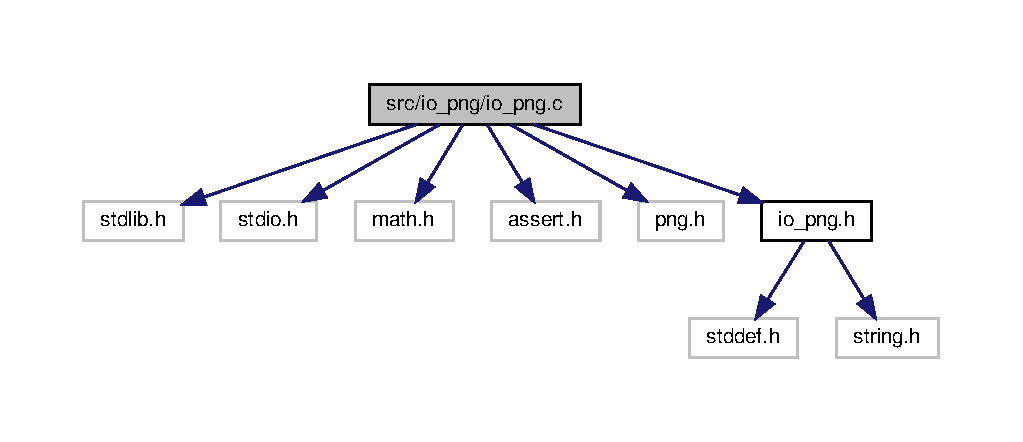
\includegraphics[width=350pt]{io__png_8c__incl}
\end{center}
\end{figure}
\subsection*{Macros}
\begin{DoxyCompactItemize}
\item 
\mbox{\Hypertarget{io__png_8c_ac4b295661ab2809e1211068b43935fff}\label{io__png_8c_ac4b295661ab2809e1211068b43935fff}} 
\#define {\bfseries P\+N\+G\+\_\+\+S\+I\+G\+\_\+\+L\+EN}~4
\item 
\mbox{\Hypertarget{io__png_8c_a59020db16c4fc483180176609389e9ed}\label{io__png_8c_a59020db16c4fc483180176609389e9ed}} 
\#define {\bfseries I\+O\+\_\+\+P\+N\+G\+\_\+\+U8}~0x0001       /$\ast$  8bit unsigned integer $\ast$/
\item 
\mbox{\Hypertarget{io__png_8c_a8b93533ae0ea6561472759cf6cbc85c0}\label{io__png_8c_a8b93533ae0ea6561472759cf6cbc85c0}} 
\#define {\bfseries I\+O\+\_\+\+P\+N\+G\+\_\+\+F32}~0x0002       /$\ast$ 32bit float $\ast$/
\end{DoxyCompactItemize}
\subsection*{Functions}
\begin{DoxyCompactItemize}
\item 
char $\ast$ \hyperlink{io__png_8c_a012b75e68d0be39dee836a3fe4ac922c}{io\+\_\+png\+\_\+info} (void)
\begin{DoxyCompactList}\small\item\em helps tracking versions, via the string tag inserted into the library \end{DoxyCompactList}\item 
unsigned char $\ast$ \hyperlink{io__png_8c_a54ce4037b9759d9a8f31c01d3315821d}{io\+\_\+png\+\_\+read\+\_\+u8} (const char $\ast$fname, size\+\_\+t $\ast$nxp, size\+\_\+t $\ast$nyp, size\+\_\+t $\ast$ncp)
\begin{DoxyCompactList}\small\item\em read a P\+NG file into a 8bit integer array \end{DoxyCompactList}\item 
unsigned char $\ast$ \hyperlink{io__png_8c_a75d4fa6df922812971d69be6d2d8c35c}{io\+\_\+png\+\_\+read\+\_\+u8\+\_\+rgb} (const char $\ast$fname, size\+\_\+t $\ast$nxp, size\+\_\+t $\ast$nyp)
\begin{DoxyCompactList}\small\item\em read a P\+NG file into a 8bit integer array, converted to R\+GB \end{DoxyCompactList}\item 
unsigned char $\ast$ \hyperlink{io__png_8c_acbe290d3529e65fdd55fd131af4713e1}{io\+\_\+png\+\_\+read\+\_\+u8\+\_\+gray} (const char $\ast$fname, size\+\_\+t $\ast$nxp, size\+\_\+t $\ast$nyp)
\begin{DoxyCompactList}\small\item\em read a P\+NG file into a 8bit integer array, converted to gray \end{DoxyCompactList}\item 
float $\ast$ \hyperlink{io__png_8c_a262d986069f1b45053769f3a5659ba10}{io\+\_\+png\+\_\+read\+\_\+f32} (const char $\ast$fname, size\+\_\+t $\ast$nxp, size\+\_\+t $\ast$nyp, size\+\_\+t $\ast$ncp)
\begin{DoxyCompactList}\small\item\em read a P\+NG file into a 32bit float array \end{DoxyCompactList}\item 
float $\ast$ \hyperlink{io__png_8c_add2a6ef684e3a42aab4f9735d16d03e8}{io\+\_\+png\+\_\+read\+\_\+f32\+\_\+rgb} (const char $\ast$fname, size\+\_\+t $\ast$nxp, size\+\_\+t $\ast$nyp)
\begin{DoxyCompactList}\small\item\em read a P\+NG file into a 32bit float array, converted to R\+GB \end{DoxyCompactList}\item 
float $\ast$ \hyperlink{io__png_8c_a7b26dc88b7f194d4d46a0599e83cafd3}{io\+\_\+png\+\_\+read\+\_\+f32\+\_\+gray} (const char $\ast$fname, size\+\_\+t $\ast$nxp, size\+\_\+t $\ast$nyp)
\begin{DoxyCompactList}\small\item\em read a P\+NG file into a 32bit float array, converted to gray \end{DoxyCompactList}\item 
int \hyperlink{io__png_8c_accb143f7e473c3c10659010bf85a7457}{io\+\_\+png\+\_\+write\+\_\+u8} (const char $\ast$fname, const unsigned char $\ast$data, size\+\_\+t nx, size\+\_\+t ny, size\+\_\+t nc)
\begin{DoxyCompactList}\small\item\em write a 8bit unsigned integer array into a P\+NG file \end{DoxyCompactList}\item 
int \hyperlink{io__png_8c_a8b49182e70dfd843d7bafbc7a5278172}{io\+\_\+png\+\_\+write\+\_\+f32} (const char $\ast$fname, const float $\ast$data, size\+\_\+t nx, size\+\_\+t ny, size\+\_\+t nc)
\begin{DoxyCompactList}\small\item\em write a float array into a P\+NG file \end{DoxyCompactList}\end{DoxyCompactItemize}


\subsection{Detailed Description}
P\+NG read/write simplified interface. 

This is a front-\/end to libpng, with routines to\+: \begin{DoxyItemize}
\item read a P\+NG file as a deinterlaced 8bit integer or float array \item write a 8bit integer or float array to a P\+NG file\end{DoxyItemize}
Multi-\/channel images are handled\+: grey, grey+alpha, rgb and rgb+alpha, as well as on-\/the-\/fly color model conversion.

\begin{DoxyRefDesc}{Todo}
\item[\hyperlink{todo__todo000001}{Todo}]handle lossless 16bit data 

add a test suite 

internally handle R\+G\+B/gray conversion in io\+\_\+png\+\_\+read\+\_\+raw() 

handle deinterlacing as a libpng transform function\end{DoxyRefDesc}


\begin{DoxyAuthor}{Author}
Nicolas Limare \href{mailto:nicolas.limare@cmla.ens-cachan.fr}{\tt nicolas.\+limare@cmla.\+ens-\/cachan.\+fr} 
\end{DoxyAuthor}


\subsection{Function Documentation}
\mbox{\Hypertarget{io__png_8c_a012b75e68d0be39dee836a3fe4ac922c}\label{io__png_8c_a012b75e68d0be39dee836a3fe4ac922c}} 
\index{io\+\_\+png.\+c@{io\+\_\+png.\+c}!io\+\_\+png\+\_\+info@{io\+\_\+png\+\_\+info}}
\index{io\+\_\+png\+\_\+info@{io\+\_\+png\+\_\+info}!io\+\_\+png.\+c@{io\+\_\+png.\+c}}
\subsubsection{\texorpdfstring{io\+\_\+png\+\_\+info()}{io\_png\_info()}}
{\footnotesize\ttfamily char$\ast$ io\+\_\+png\+\_\+info (\begin{DoxyParamCaption}\item[{void}]{ }\end{DoxyParamCaption})}



helps tracking versions, via the string tag inserted into the library 

This function is not expected to be used in real-\/world programs.

\begin{DoxyReturn}{Returns}
a pointer to a version info string 
\end{DoxyReturn}
\mbox{\Hypertarget{io__png_8c_a262d986069f1b45053769f3a5659ba10}\label{io__png_8c_a262d986069f1b45053769f3a5659ba10}} 
\index{io\+\_\+png.\+c@{io\+\_\+png.\+c}!io\+\_\+png\+\_\+read\+\_\+f32@{io\+\_\+png\+\_\+read\+\_\+f32}}
\index{io\+\_\+png\+\_\+read\+\_\+f32@{io\+\_\+png\+\_\+read\+\_\+f32}!io\+\_\+png.\+c@{io\+\_\+png.\+c}}
\subsubsection{\texorpdfstring{io\+\_\+png\+\_\+read\+\_\+f32()}{io\_png\_read\_f32()}}
{\footnotesize\ttfamily float$\ast$ io\+\_\+png\+\_\+read\+\_\+f32 (\begin{DoxyParamCaption}\item[{const char $\ast$}]{fname,  }\item[{size\+\_\+t $\ast$}]{nxp,  }\item[{size\+\_\+t $\ast$}]{nyp,  }\item[{size\+\_\+t $\ast$}]{ncp }\end{DoxyParamCaption})}



read a P\+NG file into a 32bit float array 

The array contains the deinterlaced channels. 1, 2, 4 and 8bit images are converted to float values between 0. and 1., 3., 15. or 255. 16bit images are also downscaled to 8bit before conversion.


\begin{DoxyParams}{Parameters}
{\em fname} & P\+NG file name \\
\hline
{\em nxp,nyp,ncp} & pointers to variables to be filled with the number of columns, lines and channels of the image \\
\hline
\end{DoxyParams}
\begin{DoxyReturn}{Returns}
pointer to an allocated unsigned char array of pixels, or N\+U\+LL if an error happens 
\end{DoxyReturn}
\mbox{\Hypertarget{io__png_8c_a7b26dc88b7f194d4d46a0599e83cafd3}\label{io__png_8c_a7b26dc88b7f194d4d46a0599e83cafd3}} 
\index{io\+\_\+png.\+c@{io\+\_\+png.\+c}!io\+\_\+png\+\_\+read\+\_\+f32\+\_\+gray@{io\+\_\+png\+\_\+read\+\_\+f32\+\_\+gray}}
\index{io\+\_\+png\+\_\+read\+\_\+f32\+\_\+gray@{io\+\_\+png\+\_\+read\+\_\+f32\+\_\+gray}!io\+\_\+png.\+c@{io\+\_\+png.\+c}}
\subsubsection{\texorpdfstring{io\+\_\+png\+\_\+read\+\_\+f32\+\_\+gray()}{io\_png\_read\_f32\_gray()}}
{\footnotesize\ttfamily float$\ast$ io\+\_\+png\+\_\+read\+\_\+f32\+\_\+gray (\begin{DoxyParamCaption}\item[{const char $\ast$}]{fname,  }\item[{size\+\_\+t $\ast$}]{nxp,  }\item[{size\+\_\+t $\ast$}]{nyp }\end{DoxyParamCaption})}



read a P\+NG file into a 32bit float array, converted to gray 

See \hyperlink{io__png_8c_a262d986069f1b45053769f3a5659ba10}{io\+\_\+png\+\_\+read\+\_\+f32()} for details. \mbox{\Hypertarget{io__png_8c_add2a6ef684e3a42aab4f9735d16d03e8}\label{io__png_8c_add2a6ef684e3a42aab4f9735d16d03e8}} 
\index{io\+\_\+png.\+c@{io\+\_\+png.\+c}!io\+\_\+png\+\_\+read\+\_\+f32\+\_\+rgb@{io\+\_\+png\+\_\+read\+\_\+f32\+\_\+rgb}}
\index{io\+\_\+png\+\_\+read\+\_\+f32\+\_\+rgb@{io\+\_\+png\+\_\+read\+\_\+f32\+\_\+rgb}!io\+\_\+png.\+c@{io\+\_\+png.\+c}}
\subsubsection{\texorpdfstring{io\+\_\+png\+\_\+read\+\_\+f32\+\_\+rgb()}{io\_png\_read\_f32\_rgb()}}
{\footnotesize\ttfamily float$\ast$ io\+\_\+png\+\_\+read\+\_\+f32\+\_\+rgb (\begin{DoxyParamCaption}\item[{const char $\ast$}]{fname,  }\item[{size\+\_\+t $\ast$}]{nxp,  }\item[{size\+\_\+t $\ast$}]{nyp }\end{DoxyParamCaption})}



read a P\+NG file into a 32bit float array, converted to R\+GB 

See \hyperlink{io__png_8c_a262d986069f1b45053769f3a5659ba10}{io\+\_\+png\+\_\+read\+\_\+f32()} for details. \mbox{\Hypertarget{io__png_8c_a54ce4037b9759d9a8f31c01d3315821d}\label{io__png_8c_a54ce4037b9759d9a8f31c01d3315821d}} 
\index{io\+\_\+png.\+c@{io\+\_\+png.\+c}!io\+\_\+png\+\_\+read\+\_\+u8@{io\+\_\+png\+\_\+read\+\_\+u8}}
\index{io\+\_\+png\+\_\+read\+\_\+u8@{io\+\_\+png\+\_\+read\+\_\+u8}!io\+\_\+png.\+c@{io\+\_\+png.\+c}}
\subsubsection{\texorpdfstring{io\+\_\+png\+\_\+read\+\_\+u8()}{io\_png\_read\_u8()}}
{\footnotesize\ttfamily unsigned char$\ast$ io\+\_\+png\+\_\+read\+\_\+u8 (\begin{DoxyParamCaption}\item[{const char $\ast$}]{fname,  }\item[{size\+\_\+t $\ast$}]{nxp,  }\item[{size\+\_\+t $\ast$}]{nyp,  }\item[{size\+\_\+t $\ast$}]{ncp }\end{DoxyParamCaption})}



read a P\+NG file into a 8bit integer array 

The array contains the deinterlaced channels. 1, 2 and 4bit images are converted to 8bit. 16bit images are previously downscaled to 8bit.

\begin{DoxyRefDesc}{Todo}
\item[\hyperlink{todo__todo000003}{Todo}]don\textquotesingle{}t downscale 16bit images.\end{DoxyRefDesc}



\begin{DoxyParams}{Parameters}
{\em fname} & P\+NG file name \\
\hline
{\em nxp,nyp,ncp} & pointers to variables to be filled with the number of columns, lines and channels of the image \\
\hline
\end{DoxyParams}
\begin{DoxyReturn}{Returns}
pointer to an allocated unsigned char array of pixels, or N\+U\+LL if an error happens 
\end{DoxyReturn}
\mbox{\Hypertarget{io__png_8c_acbe290d3529e65fdd55fd131af4713e1}\label{io__png_8c_acbe290d3529e65fdd55fd131af4713e1}} 
\index{io\+\_\+png.\+c@{io\+\_\+png.\+c}!io\+\_\+png\+\_\+read\+\_\+u8\+\_\+gray@{io\+\_\+png\+\_\+read\+\_\+u8\+\_\+gray}}
\index{io\+\_\+png\+\_\+read\+\_\+u8\+\_\+gray@{io\+\_\+png\+\_\+read\+\_\+u8\+\_\+gray}!io\+\_\+png.\+c@{io\+\_\+png.\+c}}
\subsubsection{\texorpdfstring{io\+\_\+png\+\_\+read\+\_\+u8\+\_\+gray()}{io\_png\_read\_u8\_gray()}}
{\footnotesize\ttfamily unsigned char$\ast$ io\+\_\+png\+\_\+read\+\_\+u8\+\_\+gray (\begin{DoxyParamCaption}\item[{const char $\ast$}]{fname,  }\item[{size\+\_\+t $\ast$}]{nxp,  }\item[{size\+\_\+t $\ast$}]{nyp }\end{DoxyParamCaption})}



read a P\+NG file into a 8bit integer array, converted to gray 

See \hyperlink{io__png_8c_a54ce4037b9759d9a8f31c01d3315821d}{io\+\_\+png\+\_\+read\+\_\+u8()} for details. \mbox{\Hypertarget{io__png_8c_a75d4fa6df922812971d69be6d2d8c35c}\label{io__png_8c_a75d4fa6df922812971d69be6d2d8c35c}} 
\index{io\+\_\+png.\+c@{io\+\_\+png.\+c}!io\+\_\+png\+\_\+read\+\_\+u8\+\_\+rgb@{io\+\_\+png\+\_\+read\+\_\+u8\+\_\+rgb}}
\index{io\+\_\+png\+\_\+read\+\_\+u8\+\_\+rgb@{io\+\_\+png\+\_\+read\+\_\+u8\+\_\+rgb}!io\+\_\+png.\+c@{io\+\_\+png.\+c}}
\subsubsection{\texorpdfstring{io\+\_\+png\+\_\+read\+\_\+u8\+\_\+rgb()}{io\_png\_read\_u8\_rgb()}}
{\footnotesize\ttfamily unsigned char$\ast$ io\+\_\+png\+\_\+read\+\_\+u8\+\_\+rgb (\begin{DoxyParamCaption}\item[{const char $\ast$}]{fname,  }\item[{size\+\_\+t $\ast$}]{nxp,  }\item[{size\+\_\+t $\ast$}]{nyp }\end{DoxyParamCaption})}



read a P\+NG file into a 8bit integer array, converted to R\+GB 

See \hyperlink{io__png_8c_a54ce4037b9759d9a8f31c01d3315821d}{io\+\_\+png\+\_\+read\+\_\+u8()} for details. \mbox{\Hypertarget{io__png_8c_a8b49182e70dfd843d7bafbc7a5278172}\label{io__png_8c_a8b49182e70dfd843d7bafbc7a5278172}} 
\index{io\+\_\+png.\+c@{io\+\_\+png.\+c}!io\+\_\+png\+\_\+write\+\_\+f32@{io\+\_\+png\+\_\+write\+\_\+f32}}
\index{io\+\_\+png\+\_\+write\+\_\+f32@{io\+\_\+png\+\_\+write\+\_\+f32}!io\+\_\+png.\+c@{io\+\_\+png.\+c}}
\subsubsection{\texorpdfstring{io\+\_\+png\+\_\+write\+\_\+f32()}{io\_png\_write\_f32()}}
{\footnotesize\ttfamily int io\+\_\+png\+\_\+write\+\_\+f32 (\begin{DoxyParamCaption}\item[{const char $\ast$}]{fname,  }\item[{const float $\ast$}]{data,  }\item[{size\+\_\+t}]{nx,  }\item[{size\+\_\+t}]{ny,  }\item[{size\+\_\+t}]{nc }\end{DoxyParamCaption})}



write a float array into a P\+NG file 

The float values are rounded to 8bit integers, and bounded to \mbox{[}0, 255\mbox{]}.

\begin{DoxyRefDesc}{Todo}
\item[\hyperlink{todo__todo000005}{Todo}]handle 16bit images and flexible min/max\end{DoxyRefDesc}



\begin{DoxyParams}{Parameters}
{\em fname} & P\+NG file name \\
\hline
{\em data} & array to write \\
\hline
{\em nx,ny,nc} & number of columns, lines and channels of the image \\
\hline
\end{DoxyParams}
\begin{DoxyReturn}{Returns}
0 if everything OK, -\/1 if an error occured 
\end{DoxyReturn}
\mbox{\Hypertarget{io__png_8c_accb143f7e473c3c10659010bf85a7457}\label{io__png_8c_accb143f7e473c3c10659010bf85a7457}} 
\index{io\+\_\+png.\+c@{io\+\_\+png.\+c}!io\+\_\+png\+\_\+write\+\_\+u8@{io\+\_\+png\+\_\+write\+\_\+u8}}
\index{io\+\_\+png\+\_\+write\+\_\+u8@{io\+\_\+png\+\_\+write\+\_\+u8}!io\+\_\+png.\+c@{io\+\_\+png.\+c}}
\subsubsection{\texorpdfstring{io\+\_\+png\+\_\+write\+\_\+u8()}{io\_png\_write\_u8()}}
{\footnotesize\ttfamily int io\+\_\+png\+\_\+write\+\_\+u8 (\begin{DoxyParamCaption}\item[{const char $\ast$}]{fname,  }\item[{const unsigned char $\ast$}]{data,  }\item[{size\+\_\+t}]{nx,  }\item[{size\+\_\+t}]{ny,  }\item[{size\+\_\+t}]{nc }\end{DoxyParamCaption})}



write a 8bit unsigned integer array into a P\+NG file 


\begin{DoxyParams}{Parameters}
{\em fname} & P\+NG file name \\
\hline
{\em data} & array to write \\
\hline
{\em nx,ny,nc} & number of columns, lines and channels of the image \\
\hline
\end{DoxyParams}
\begin{DoxyReturn}{Returns}
0 if everything OK, -\/1 if an error occured 
\end{DoxyReturn}

\hypertarget{meanshift_8cpp}{}\section{src/meanshift.cpp File Reference}
\label{meanshift_8cpp}\index{src/meanshift.\+cpp@{src/meanshift.\+cpp}}


Main program for Meanshift segmentation.  


{\ttfamily \#include $<$stdio.\+h$>$}\newline
{\ttfamily \#include $<$cstdlib$>$}\newline
{\ttfamily \#include \char`\"{}ms/ms.\+h\char`\"{}}\newline
{\ttfamily \#include \char`\"{}io\+\_\+png/io\+\_\+png.\+h\char`\"{}}\newline
Include dependency graph for meanshift.\+cpp\+:\nopagebreak
\begin{figure}[H]
\begin{center}
\leavevmode
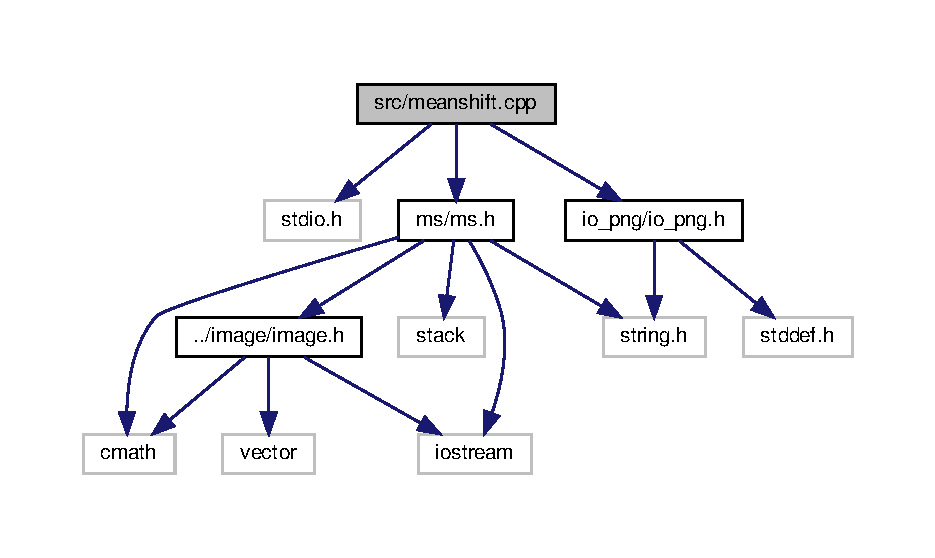
\includegraphics[width=350pt]{meanshift_8cpp__incl}
\end{center}
\end{figure}
\subsection*{Functions}
\begin{DoxyCompactItemize}
\item 
\mbox{\Hypertarget{meanshift_8cpp_a0ddf1224851353fc92bfbff6f499fa97}\label{meanshift_8cpp_a0ddf1224851353fc92bfbff6f499fa97}} 
int {\bfseries main} (int argc, char $\ast$argv\mbox{[}$\,$\mbox{]})
\end{DoxyCompactItemize}


\subsection{Detailed Description}
Main program for Meanshift segmentation. 

\begin{DoxyAuthor}{Author}
Damir Demirović \href{mailto:damir.demirovic@untz.ba}{\tt damir.\+demirovic@untz.\+ba} 
\end{DoxyAuthor}

\hypertarget{ms_8cpp}{}\section{src/ms/ms.cpp File Reference}
\label{ms_8cpp}\index{src/ms/ms.\+cpp@{src/ms/ms.\+cpp}}


Functions for Meanshift algorithm.  


{\ttfamily \#include \char`\"{}ms.\+h\char`\"{}}\newline
{\ttfamily \#include $<$stack$>$}\newline
{\ttfamily \#include \char`\"{}../ra/\+Transitive\+Closure.\+h\char`\"{}}\newline
Include dependency graph for ms.\+cpp\+:\nopagebreak
\begin{figure}[H]
\begin{center}
\leavevmode
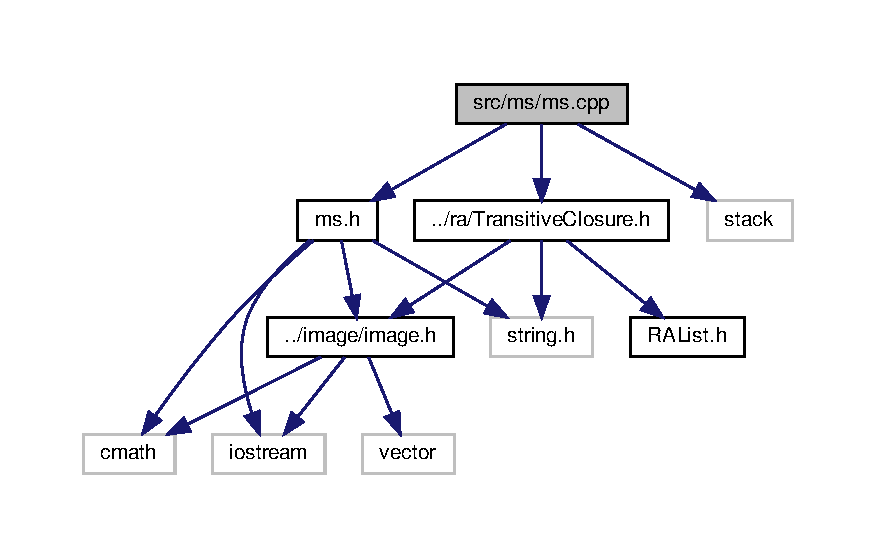
\includegraphics[width=350pt]{ms_8cpp__incl}
\end{center}
\end{figure}
\subsection*{Functions}
\begin{DoxyCompactItemize}
\item 
void \hyperlink{ms_8cpp_a1236189e7ed18bfff1ec1abc02de7737}{Add\+To\+Stack} (std\+::stack$<$ \hyperlink{structMSPoint}{M\+S\+Point} $>$ \&stack, int i, int j)
\begin{DoxyCompactList}\small\item\em Function Add\+To\+Stack add point to the stack. \end{DoxyCompactList}\item 
uchar $\ast$ \hyperlink{ms_8cpp_aa65ad2ef8d04df108ecdf3324a664c7f}{Mean\+Shift} (uchar $\ast$image, uchar $\ast$filtered\+\_\+luv, int $\ast$$\ast$labels, int width, int height, int spatial\+\_\+radius, double color\+\_\+radius, int min\+Region, int num\+\_\+iters)
\begin{DoxyCompactList}\small\item\em Function Mean\+Shift runs two phases of Mean shift algorithm Filter and Segment using Meanshift algorithm The main program for Meanshift Meanshift algorithm\+: First phase is image filtering. Filtered image is in L$\ast$u$\ast$v colorspace Second phase is image segmentation. \end{DoxyCompactList}\item 
uchar $\ast$ \hyperlink{ms_8cpp_a3838214793438d3ada3662f11be936a1}{M\+S\+\_\+\+Filter} (uchar $\ast$image, int width, int height, int spatial\+\_\+radius, double color\+\_\+radius, int init\+Iters)
\begin{DoxyCompactList}\small\item\em Function M\+S\+\_\+\+Filter filter image usign Meanshift algorithm using a circular flat kernel and color distance in L$\ast$u$\ast$v colorspace. \end{DoxyCompactList}\item 
int \hyperlink{ms_8cpp_a20fca730748cd5586b1f86724d4a8f24}{M\+S\+\_\+\+Segment} (uchar $\ast$image, int width, int height, int $\ast$$\ast$labels, double color\+\_\+radius, int min\+Region)
\begin{DoxyCompactList}\small\item\em Function M\+S\+\_\+\+Segment segments the image using Meanshift algorithm. \end{DoxyCompactList}\item 
int \hyperlink{ms_8cpp_ad0123962474a1abc05771296d5c1d622}{M\+S\+\_\+\+Cluster} (uchar $\ast$image, int width, int height, int $\ast$$\ast$labels, int $\ast$mode\+Points, float $\ast$mode, double color\+\_\+radius)
\begin{DoxyCompactList}\small\item\em Function M\+S\+\_\+\+Cluster cluster the image using Meanshift. \end{DoxyCompactList}\end{DoxyCompactItemize}


\subsection{Detailed Description}
Functions for Meanshift algorithm. 

\begin{DoxyAuthor}{Author}
Damir Demirović \href{mailto:damir.demirovic@untz.ba}{\tt damir.\+demirovic@untz.\+ba} 
\end{DoxyAuthor}


\subsection{Function Documentation}
\mbox{\Hypertarget{ms_8cpp_a1236189e7ed18bfff1ec1abc02de7737}\label{ms_8cpp_a1236189e7ed18bfff1ec1abc02de7737}} 
\index{ms.\+cpp@{ms.\+cpp}!Add\+To\+Stack@{Add\+To\+Stack}}
\index{Add\+To\+Stack@{Add\+To\+Stack}!ms.\+cpp@{ms.\+cpp}}
\subsubsection{\texorpdfstring{Add\+To\+Stack()}{AddToStack()}}
{\footnotesize\ttfamily void Add\+To\+Stack (\begin{DoxyParamCaption}\item[{std\+::stack$<$ \hyperlink{structMSPoint}{M\+S\+Point} $>$ \&}]{stack,  }\item[{int}]{i,  }\item[{int}]{j }\end{DoxyParamCaption})}



Function Add\+To\+Stack add point to the stack. 


\begin{DoxyParams}{Parameters}
{\em i} & x coordinate of the point \\
\hline
{\em j} & y coordinate of the point \\
\hline
\end{DoxyParams}
\mbox{\Hypertarget{ms_8cpp_aa65ad2ef8d04df108ecdf3324a664c7f}\label{ms_8cpp_aa65ad2ef8d04df108ecdf3324a664c7f}} 
\index{ms.\+cpp@{ms.\+cpp}!Mean\+Shift@{Mean\+Shift}}
\index{Mean\+Shift@{Mean\+Shift}!ms.\+cpp@{ms.\+cpp}}
\subsubsection{\texorpdfstring{Mean\+Shift()}{MeanShift()}}
{\footnotesize\ttfamily uchar$\ast$ Mean\+Shift (\begin{DoxyParamCaption}\item[{uchar $\ast$}]{image,  }\item[{uchar $\ast$}]{filtered\+\_\+luv,  }\item[{int $\ast$$\ast$}]{labels,  }\item[{int}]{width,  }\item[{int}]{height,  }\item[{int}]{spatial\+\_\+radius,  }\item[{double}]{color\+\_\+radius,  }\item[{int}]{min\+Region,  }\item[{int}]{num\+\_\+iters }\end{DoxyParamCaption})}



Function Mean\+Shift runs two phases of Mean shift algorithm Filter and Segment using Meanshift algorithm The main program for Meanshift Meanshift algorithm\+: First phase is image filtering. Filtered image is in L$\ast$u$\ast$v colorspace Second phase is image segmentation. 


\begin{DoxyParams}{Parameters}
{\em image} & input image for Meanshift algorithm \\
\hline
{\em filtered\+\_\+luv} & output image filtered with Meanshift algorithm \\
\hline
{\em labels} & labels \\
\hline
{\em width} & width of the image \\
\hline
{\em height} & height of the image \\
\hline
{\em spatial\+\_\+radius} & spatial radius \\
\hline
{\em color\+\_\+radius} & range radius \\
\hline
{\em min\+Region} & minimal region for merging \\
\hline
{\em num\+\_\+iters} & initial number of iterations \\
\hline
\end{DoxyParams}
\begin{DoxyReturn}{Returns}
segmented image 
\end{DoxyReturn}
\mbox{\Hypertarget{ms_8cpp_ad0123962474a1abc05771296d5c1d622}\label{ms_8cpp_ad0123962474a1abc05771296d5c1d622}} 
\index{ms.\+cpp@{ms.\+cpp}!M\+S\+\_\+\+Cluster@{M\+S\+\_\+\+Cluster}}
\index{M\+S\+\_\+\+Cluster@{M\+S\+\_\+\+Cluster}!ms.\+cpp@{ms.\+cpp}}
\subsubsection{\texorpdfstring{M\+S\+\_\+\+Cluster()}{MS\_Cluster()}}
{\footnotesize\ttfamily int M\+S\+\_\+\+Cluster (\begin{DoxyParamCaption}\item[{uchar $\ast$}]{image,  }\item[{int}]{width,  }\item[{int}]{height,  }\item[{int $\ast$$\ast$}]{labels,  }\item[{int $\ast$}]{mode\+Points,  }\item[{float $\ast$}]{mode,  }\item[{double}]{color\+\_\+radius }\end{DoxyParamCaption})}



Function M\+S\+\_\+\+Cluster cluster the image using Meanshift. 


\begin{DoxyParams}{Parameters}
{\em image} & in L$\ast$u$\ast$v colorspace, \\
\hline
{\em width} & width of the image \\
\hline
{\em height} & height of the image \\
\hline
{\em labels} & contain labels \\
\hline
{\em mode\+Points} & data about mode points \\
\hline
{\em mode} & data about mode \\
\hline
{\em color\+\_\+radius} & range radius \\
\hline
\end{DoxyParams}
\begin{DoxyReturn}{Returns}
reg\+Count number of regions 
\end{DoxyReturn}
\mbox{\Hypertarget{ms_8cpp_a3838214793438d3ada3662f11be936a1}\label{ms_8cpp_a3838214793438d3ada3662f11be936a1}} 
\index{ms.\+cpp@{ms.\+cpp}!M\+S\+\_\+\+Filter@{M\+S\+\_\+\+Filter}}
\index{M\+S\+\_\+\+Filter@{M\+S\+\_\+\+Filter}!ms.\+cpp@{ms.\+cpp}}
\subsubsection{\texorpdfstring{M\+S\+\_\+\+Filter()}{MS\_Filter()}}
{\footnotesize\ttfamily uchar$\ast$ M\+S\+\_\+\+Filter (\begin{DoxyParamCaption}\item[{uchar $\ast$}]{image,  }\item[{int}]{width,  }\item[{int}]{height,  }\item[{int}]{spatial\+\_\+radius,  }\item[{double}]{color\+\_\+radius,  }\item[{int}]{init\+Iters }\end{DoxyParamCaption})}



Function M\+S\+\_\+\+Filter filter image usign Meanshift algorithm using a circular flat kernel and color distance in L$\ast$u$\ast$v colorspace. 

Based on implementation from \href{https://imagej.nih.gov/ij/plugins/download/Mean_Shift.java}{\tt https\+://imagej.\+nih.\+gov/ij/plugins/download/\+Mean\+\_\+\+Shift.\+java}

For each pixel of the image and the set ot the neighboring pixels within the specified spatial radius and color distance is determined. For this set of neighbor pixels, the new spatial center an the new color mean values are calculated. These new values will serve as the new center for the next iteration. This procedure will iterate until the spatial and color means will stop changing or the maximal number of iterations is achieved.


\begin{DoxyParams}{Parameters}
{\em image} & input image \\
\hline
{\em width} & width of the image \\
\hline
{\em height} & height of the image \\
\hline
{\em spatial\+\_\+radius} & spatial radius \\
\hline
{\em color\+\_\+radius} & range radius \\
\hline
{\em init\+Iters} & initial number of iterations \\
\hline
\end{DoxyParams}
\begin{DoxyReturn}{Returns}
luv Meanshift filtered image in L$\ast$u$\ast$v colorspace. 
\end{DoxyReturn}
\mbox{\Hypertarget{ms_8cpp_a20fca730748cd5586b1f86724d4a8f24}\label{ms_8cpp_a20fca730748cd5586b1f86724d4a8f24}} 
\index{ms.\+cpp@{ms.\+cpp}!M\+S\+\_\+\+Segment@{M\+S\+\_\+\+Segment}}
\index{M\+S\+\_\+\+Segment@{M\+S\+\_\+\+Segment}!ms.\+cpp@{ms.\+cpp}}
\subsubsection{\texorpdfstring{M\+S\+\_\+\+Segment()}{MS\_Segment()}}
{\footnotesize\ttfamily int M\+S\+\_\+\+Segment (\begin{DoxyParamCaption}\item[{uchar $\ast$}]{image,  }\item[{int}]{width,  }\item[{int}]{height,  }\item[{int $\ast$$\ast$}]{labels,  }\item[{double}]{color\+\_\+radius,  }\item[{int}]{min\+Region }\end{DoxyParamCaption})}



Function M\+S\+\_\+\+Segment segments the image using Meanshift algorithm. 


\begin{DoxyParams}{Parameters}
{\em image} & in L$\ast$u$\ast$v colorspace, \\
\hline
{\em width} & width of the image \\
\hline
{\em height} & height of the image \\
\hline
{\em labels} & contain labels \\
\hline
{\em color\+\_\+radius} & range radius \\
\hline
{\em min\+Region} & minimal region for merging \\
\hline
\end{DoxyParams}
\begin{DoxyReturn}{Returns}
reg\+Count Number of segmented regions 
\end{DoxyReturn}

\hypertarget{msfilter_8cpp}{}\section{src/msfilter.cpp File Reference}
\label{msfilter_8cpp}\index{src/msfilter.\+cpp@{src/msfilter.\+cpp}}


Main program for Meanshift filtering.  


{\ttfamily \#include $<$stdio.\+h$>$}\newline
{\ttfamily \#include $<$cstdlib$>$}\newline
{\ttfamily \#include \char`\"{}ms/ms.\+h\char`\"{}}\newline
{\ttfamily \#include \char`\"{}io\+\_\+png/io\+\_\+png.\+h\char`\"{}}\newline
Include dependency graph for msfilter.\+cpp\+:\nopagebreak
\begin{figure}[H]
\begin{center}
\leavevmode
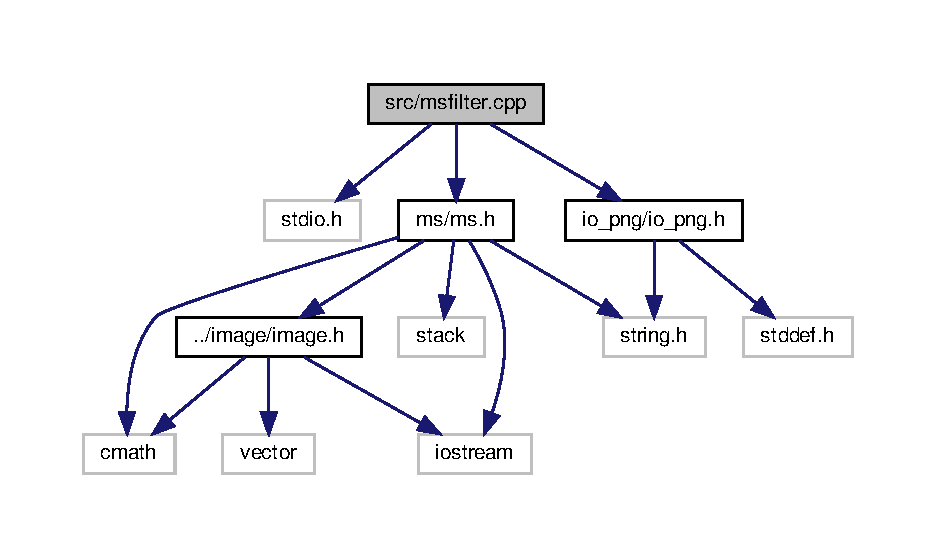
\includegraphics[width=350pt]{msfilter_8cpp__incl}
\end{center}
\end{figure}
\subsection*{Functions}
\begin{DoxyCompactItemize}
\item 
\mbox{\Hypertarget{msfilter_8cpp_a0ddf1224851353fc92bfbff6f499fa97}\label{msfilter_8cpp_a0ddf1224851353fc92bfbff6f499fa97}} 
int {\bfseries main} (int argc, char $\ast$argv\mbox{[}$\,$\mbox{]})
\end{DoxyCompactItemize}


\subsection{Detailed Description}
Main program for Meanshift filtering. 

\begin{DoxyAuthor}{Author}
Damir Demirović \href{mailto:damir.demirovic@untz.ba}{\tt damir.\+demirovic@untz.\+ba} 
\end{DoxyAuthor}

%--- End generated contents ---

% Index
\backmatter
\newpage
\phantomsection
\clearemptydoublepage
\addcontentsline{toc}{chapter}{Index}
\printindex

\end{document}
